\chapter{Testing}
\label{ch:testing}

\section{Test strategy}

In the first version of this thesis only the worker had automated tests, and the system tests were a list of steps I carried out by hand before each demonstration. That was not enough: a change to the queue or to the results format could break the platform without any test noticing.

The testing now works on five levels, and the first four run on every push in the CI pipeline (\autoref{sec:cicd}). Static checks come first: the TypeScript compiler checks the API and the dashboard, and oxlint lints the dashboard. White-box unit tests then check the worker's algorithms with constructed data whose correct result is known (43 tests) and the dashboard's overlay mathematics (23 tests). The backend's 42 API tests send real HTTP requests to the application, which talks to a real PostgreSQL test database and Redis. The 11 black-box system tests treat the whole platform in Docker as a browser would, through nginx, the REST API and the WebSocket, and include a real analysis. The fifth level is measurement: an accuracy check against hand-annotated frames, the analysis of the five demo clips and of two full halves, and processing-time comparisons.

A change that breaks any of the first four levels cannot be published as a Docker image, because the images job only runs after all of them pass.

\section{Unit tests of the worker}

The worker's tests are in \texttt{worker/tests/} and run with \texttt{python -m pytest} in about 10 seconds. They need neither videos nor model files: a known camera matrix is used to project pitch landmarks into a synthetic image, a red or lime shirt is painted on grass, a player is made to run in a straight line. Parametrised tests repeat a check for every formation. Most of the tests written after the first version are regression tests: each reproduces a defect found on real footage, so it cannot return silently. \autoref{tab:worker-tests} lists them; all 43 pass.

\begin{longtable}{|p{0.42\textwidth}|p{0.05\textwidth}|p{0.43\textwidth}|}
	\hline
	\textbf{Test} & \textbf{Cases} & \textbf{What is checked} \\
	\hline
	\endhead
	\multicolumn{3}{|l|}{\textit{Homography} (\texttt{test\_\allowbreak{}homography.\allowbreak{}py})} \\
	\hline
	\texttt{pitch\_\allowbreak{}keypoints\_\allowbreak{}match\_\allowbreak{}standard\_\allowbreak{}dimensions} & 1 & The 32 landmarks span exactly 0--105\,m and 0--68\,m. \\
	\hline
	\texttt{fit\_\allowbreak{}recovers\_\allowbreak{}the\_\allowbreak{}true\_\allowbreak{}mapping} & 1 & From 8 exact pairs all are inliers, the error is below 1\,mm, new points are projected right. \\
	\hline
	\texttt{fit\_\allowbreak{}ignores\_\allowbreak{}a\_\allowbreak{}wrong\_\allowbreak{}keypoint} & 1 & A landmark moved by 470\,px is rejected by RANSAC (\autoref{code:unit-test}). \\
	\hline
	\texttt{collinear\_\allowbreak{}keypoints\_\allowbreak{}are\_\allowbreak{}rejected} & 1 & Four points on the halfway line give no homography. \\
	\hline
	\texttt{project\_\allowbreak{}tracks\_\allowbreak{}puts\_\allowbreak{}feet\_\allowbreak{}on\_\allowbreak{}the\_\allowbreak{}pitch} & 1 & A foot at the image of the centre spot lands at (52.5, 34.0)\,m. \\
	\hline
	\texttt{exported\_\allowbreak{}matrices\_\allowbreak{}are\_\allowbreak{}finite\_\allowbreak{}when\_\allowbreak{}last\_\allowbreak{}entry\_\allowbreak{}is\_\allowbreak{}zero} & 1 & Regression: no \texttt{NaN} when the last matrix element is 0. \\
	\hline
	\texttt{smoothing\_\allowbreak{}removes\_\allowbreak{}a\_\allowbreak{}one\_\allowbreak{}frame\_\allowbreak{}wobble\_\allowbreak{}but\_\allowbreak{}follows\_\allowbreak{}a\_\allowbreak{}camera\_\allowbreak{}pan} & 1 & A 5\,m wobble in one frame disappears, a steady pan is still followed. \\
	\hline
	\multicolumn{3}{|l|}{\textit{Teams, formations and positions} (\texttt{test\_\allowbreak{}clustering.\allowbreak{}py}, \texttt{test\_\allowbreak{}positions.\allowbreak{}py})} \\
	\hline
	\texttt{shirt\_\allowbreak{}colour\_\allowbreak{}is\_\allowbreak{}measured\_\allowbreak{}with\_\allowbreak{}local\_\allowbreak{}grass} & 2 & A red and a lime shirt on grass are measured within 5 Lab units. \\
	\hline
	\texttt{fixed\_\allowbreak{}green\_\allowbreak{}range\_\allowbreak{}loses\_\allowbreak{}green\_\allowbreak{}kits} & 1 & Documents the old defect: a fixed green range removes the lime shirt. \\
	\hline
	\texttt{formation\_\allowbreak{}templates\_\allowbreak{}have\_\allowbreak{}ten\_\allowbreak{}outfield\_\allowbreak{}players} & 9 & Every template has 10 slots. \\
	\hline
	\texttt{noisy\_\allowbreak{}formation\_\allowbreak{}is\_\allowbreak{}recognised} & 9 & Each formation, scaled to a $35 \times 50$\,m shape with 1.5\,m noise per player, is matched to the right template. \\
	\hline
	\texttt{slot\_\allowbreak{}names\_\allowbreak{}match\_\allowbreak{}the\_\allowbreak{}template\_\allowbreak{}order} & 1 & Position names come out in template order (right to left per line). \\
	\hline
	\texttt{a\_\allowbreak{}player\_\allowbreak{}wearing\_\allowbreak{}the\_\allowbreak{}referee\_\allowbreak{}kit\_\allowbreak{}is\_\allowbreak{}found} & 1 & A ``player'' in the referees' colour is found as a referee. \\
	\hline
	\texttt{a\_\allowbreak{}goalkeeper\_\allowbreak{}in\_\allowbreak{}their\_\allowbreak{}box\_\allowbreak{}stays\_\allowbreak{}a\_\allowbreak{}goalkeeper} & 1 & Regression: a goalkeeper in an unusual kit inside the box is not turned into a referee; one in midfield is. \\
	\hline
	\multicolumn{3}{|l|}{\textit{Clean-up} (\texttt{test\_\allowbreak{}cleanup.\allowbreak{}py})} \\
	\hline
	\texttt{people\_\allowbreak{}standing\_\allowbreak{}off\_\allowbreak{}the\_\allowbreak{}pitch\_\allowbreak{}are\_\allowbreak{}removed\_\allowbreak{}but\_\allowbreak{}not\_\allowbreak{}a\_\allowbreak{}throw\_\allowbreak{}in} & 1 & A coach 3\,m off the pitch is removed; a winger stepping out briefly and an assistant referee stay. \\
	\hline
	\texttt{spare\_\allowbreak{}ball\_\allowbreak{}off\_\allowbreak{}the\_\allowbreak{}pitch\_\allowbreak{}is\_\allowbreak{}ignored\_\allowbreak{}and\_\allowbreak{}the\_\allowbreak{}ball\_\allowbreak{}path\_\allowbreak{}is\_\allowbreak{}followed} & 1 & With a rolling ball, a sharper spare ball off the pitch and a distant object, the rolling ball is chosen in every frame. \\
	\hline
	\texttt{penalty\_\allowbreak{}spot\_\allowbreak{}is\_\allowbreak{}not\_\allowbreak{}taken\_\allowbreak{}as\_\allowbreak{}the\_\allowbreak{}ball} & 1 & A confident ``ball'' on the penalty spot loses to a real one. \\
	\hline
	\texttt{two\_\allowbreak{}pieces\_\allowbreak{}of\_\allowbreak{}one\_\allowbreak{}player\_\allowbreak{}are\_\allowbreak{}joined\_\allowbreak{}and\_\allowbreak{}renumbered} & 1 & Two nearby pieces are joined, a distant one is not, IDs start at 1. \\
	\hline
	\multicolumn{3}{|l|}{\textit{Trajectories, metrics and export} (\texttt{test\_\allowbreak{}export.\allowbreak{}py}, \texttt{test\_\allowbreak{}metrics.\allowbreak{}py})} \\
	\hline
	\texttt{non\_\allowbreak{}finite\_\allowbreak{}numbers\_\allowbreak{}become\_\allowbreak{}null} & 1 & \texttt{NaN} and infinity become \texttt{null} and the atomic write succeeds. \\
	\hline
	\texttt{short\_\allowbreak{}ball\_\allowbreak{}gaps\_\allowbreak{}are\_\allowbreak{}interpolated} & 1 & A ball seen in frames 0 and 6 is filled in at frames 2 and 4. \\
	\hline
	\texttt{smoothing\_\allowbreak{}keeps\_\allowbreak{}raw\_\allowbreak{}positions\_\allowbreak{}and\_\allowbreak{}reduces\_\allowbreak{}jitter} & 1 & A $\pm 1$\,m zig-zag becomes an average step below 0.5\,m. \\
	\hline
	\texttt{steady\_\allowbreak{}run\_\allowbreak{}gives\_\allowbreak{}the\_\allowbreak{}true\_\allowbreak{}speed} & 1 & A 7\,m/s run gives 25.2\,km/h and the right distance. \\
	\hline
	\texttt{one\_\allowbreak{}position\_\allowbreak{}jump\_\allowbreak{}does\_\allowbreak{}not\_\allowbreak{}create\_\allowbreak{}a\_\allowbreak{}fake\_\allowbreak{}sprint} & 1 & Regression: a 0.35\,m jump keeps the top speed below 27\,km/h. \\
	\hline
	\texttt{tracks\_\allowbreak{}shorter\_\allowbreak{}than\_\allowbreak{}a\_\allowbreak{}second\_\allowbreak{}have\_\allowbreak{}no\_\allowbreak{}top\_\allowbreak{}speed} & 1 & A track under one second gets no top speed. \\
	\hline
	\multicolumn{3}{|l|}{\textit{Queue worker and GPU client} (\texttt{test\_\allowbreak{}worker.\allowbreak{}py}, \texttt{test\_\allowbreak{}remote.\allowbreak{}py})} \\
	\hline
	\texttt{a\_\allowbreak{}job\_\allowbreak{}handed\_\allowbreak{}out\_\allowbreak{}again\_\allowbreak{}after\_\allowbreak{}sleep\_\allowbreak{}is\_\allowbreak{}not\_\allowbreak{}analysed\_\allowbreak{}twice} & 1 & Regression: the same job twice runs once; a re-analysis runs again. \\
	\hline
	\texttt{cancelling\_\allowbreak{}tells\_\allowbreak{}the\_\allowbreak{}gpu\_\allowbreak{}service\_\allowbreak{}to\_\allowbreak{}stop} & 1 & Against a pretend GPU service: cancel calls \texttt{/cancel} and downloads nothing. \\
	\hline
	\caption{Unit tests of the worker (test names without the \texttt{test\_\allowbreak{}} prefix)}
	\label{tab:worker-tests}
\end{longtable}

\begin{lstlisting}[language=Python, caption={A unit test of the RANSAC fit (from \texttt{worker/tests/test\_\allowbreak{}homography.\allowbreak{}py})}, label={code:unit-test}]
def test_fit_ignores_a_wrong_keypoint():
    pitch_points = PitchDimensions().keypoints[[0, 5, 13, 16, 9, 12, 30, 31]]
    image_points = to_image(pitch_points)
    image_points[3] += [400, -250]  # one badly detected landmark
    homography = Homography.fit(image_points, pitch_points)
    assert homography is not None and homography.n_inliers == len(pitch_points) - 1
\end{lstlisting}

\section{API tests of the backend}

The backend's tests in \texttt{backend/test/} use Vitest~\cite{vitest} and SuperTest~\cite{supertest}, which sends real HTTP requests to the Express application without starting a server. I decided against mocking the database: most bugs I had found in the API were about how routes, Prisma and BullMQ work together, and a mock would have hidden exactly those. The tests therefore run against a real PostgreSQL database, the normal one with \texttt{\_\allowbreak{}test} added to its name, which Prisma's migrations create before the first test. They use Redis database 1, so the real worker, which listens on database 0, never picks up a test upload, a temporary storage folder, and an upload limit of 1\,MB so that the ``too large'' test is fast. Before every test, the tables are emptied and the test queue is cleared, and the tests run one file at a time because they share the database. A SuperTest agent works like a browser: it keeps the log-in cookie between requests. The 42 tests (\autoref{tab:api-tests}) take about 30 seconds.

\begin{longtable}{|p{0.25\textwidth}|p{0.66\textwidth}|}
	\hline
	\textbf{Group} & \textbf{What is tested} \\
	\hline
	\endhead
	Registration (6) & Creates the account and logs in without returning the password; stores a bcrypt hash; refuses an existing e-mail regardless of case; refuses a short password, an invalid address and a missing name with a message naming the field. \\
	\hline
	Log-in and log-out (4) & Right password works; wrong password and unknown e-mail get the same answer; \texttt{/auth/me} knows the user until log-out; a forged cookie is rejected. \\
	\hline
	Uploading (7) & Only when logged in; stores the file, creates a queued match and a job whose ID is the match ID; refuses a missing file, non-video names and types, a text file disguised as \texttt{.\allowbreak{}mp4} (and deletes it), files over the limit, an unknown mode. \\
	\hline
	Other users' matches (1) & Every route, including cancel, answers 404 for another user's match; their list stays empty. \\
	\hline
	Rules during analysis (4) & Results and reports only after the analysis; no double queueing; no deleting while processing; re-analysis in another mode. \\
	\hline
	Deleting (1) & Removes the match, its waiting job and its video file. \\
	\hline
	Cancelling (4) & A queued analysis is cancelled at once and leaves the queue; a running one (a test worker holds the job) gets the cancel note in Redis; refused when nothing runs and for other users; a cancelled re-analysis returns to the earlier results. \\
	\hline
	Coaching report (10) & Reports ``not configured'' without Azure settings; eight measured kit colours get the right names; the model's input names colours and positions and contains no colour codes or ``Player \#''. \\
	\hline
	Platform (5) & The health check reaches the database and Redis; unknown API paths answer 404 in JSON; stored paths cannot leave the storage folder; files are recognised as videos by their first bytes. \\
	\hline
	\caption{API tests of the backend (number of tests in brackets)}
	\label{tab:api-tests}
\end{longtable}

\section{Unit tests of the dashboard}

The overlay mathematics lives in two pure modules, \texttt{geometry.\allowbreak{}ts} and \texttt{timeline.\allowbreak{}ts}, which have no dependency on React or the browser, so Vitest tests them directly with small hand-made results files. The 23 tests cover \texttt{applyHomography} (identity, scale and offset, perspective division, points behind the camera), \texttt{lerpHomography}, \texttt{convexHull} (outer points only, points on an edge, fewer than three points), \texttt{fitContain} for wide and tall boxes, and the \texttt{Timeline}: the exact state at an analysed frame, interpolation halfway between two, the ball with an unknown pitch position, never blending across a long gap, the movement path, the ball path that stops at a missing ball, \texttt{indexAt}, and, for version-3 results, position labels, REF for referees, blank labels for unknown positions and a position's path split where another player takes over.

\section{System tests}

The system tests in \texttt{tests/system/} test the running platform from the outside, through nginx on port 8080, exactly as a browser does: \texttt{httpx} for the REST API and \texttt{python-socketio} for the live updates. Nothing is mocked, so a passing run means that the frontend server, the API, the database, the queue and the worker really work together. In CI the system job starts the whole platform with Docker Compose and runs them; locally they run against the platform on the laptop in about 11 minutes, most of it a real CPU analysis of a 3-second clip. \autoref{tab:system-tests} lists them; all pass.

\begin{longtable}{|p{0.04\textwidth}|p{0.27\textwidth}|p{0.30\textwidth}|p{0.27\textwidth}|}
	\hline
	\textbf{\#} & \textbf{Test} & \textbf{Action} & \textbf{Expected and observed} \\
	\hline
	\endhead
	1 & Health check & GET \texttt{/api/health} & 200, database and Redis up, at least 1 worker \\
	\hline
	2 & Deep link & Open \texttt{/matches/<id>} directly & nginx serves the dashboard \\
	\hline
	3 & Unknown API path & GET \texttt{/api/nothing} & 404 with a JSON error \\
	\hline
	4 & Login required & GET \texttt{/api/matches} without cookie & 401 \\
	\hline
	5--6 & Invalid registrations & Short password; invalid e-mail & 400 naming the field \\
	\hline
	7 & Log-in and log-out & Register, \texttt{/auth/me}, log out, \texttt{/auth/me} & 201, 200, 204, 401 \\
	\hline
	8 & Non-videos refused & A text file, and a text file named \texttt{.\allowbreak{}mp4} & 400 for both \\
	\hline
	9 & Video without players & A real 2-second video of plain grass & First attempt fails, retry, then failed with ``No players were detected in this video'' \\
	\hline
	10 & Full analysis & Upload a 3-second Bundesliga clip in Quick mode and listen on the WebSocket & At least 5 live updates with rising progress up to 100; completed with both teams; results version 3 with position labels; video Range request answers 206; another user gets 404; re-analyse works; delete works \\
	\hline
	11 & Cancelling & Upload two clips; cancel the queued one, then the running one & Queued: cancelled at once. Running: ``Cancelling\dots'', then cancelled within 60\,s (observed: 4\,s); both can be deleted \\
	\hline
	\caption{System tests}
	\label{tab:system-tests}
\end{longtable}

The dashboard's drawing was checked by hand in Edge and Chrome, and the screenshots of \autoref{ch:user} were captured by a Playwright~\cite{playwright} script that walks through the same steps: playing, pausing and stepping frames with every layer and heatmap switched on, selecting players on the video and the board, entering and leaving full screen, generating the coaching report, and the cancel, failure and delete flows.

\section{Accuracy against hand-annotated frames}
\label{sec:accuracy}

The first version of the thesis judged correctness only by internal measures and by watching the overlays. For a quantitative check I annotated 20 frames by hand: four from each demo clip, at 15, 40, 65 and 90\,\% of its analysed frames. The script \texttt{tests/accuracy/extract\_\allowbreak{}frames.\allowbreak{}py} saves exactly the frames the worker analysed, and \texttt{annotate.\allowbreak{}html}, a small page I wrote for the purpose, lets the annotator click every person's feet with a label (Team 1, Team 2, goalkeeper or referee), the ball and visible pitch landmarks. A person whose feet are hidden behind another player is clicked where the feet would be; a person of whom only a head or an arm is visible is skipped. The 20 frames contain 466 annotated people.

\texttt{evaluate.\allowbreak{}py} then compares the annotations with the results files. Clicked feet are paired with detected foot points by the Hungarian algorithm, and a pair counts if it is closer than 35 pixels at 1080p. Team labels are compared under the better of the two possible assignments of ``Team 1'' and ``Team 2'' to the system's teams, per clip. The ball counts as found within 20 pixels. Clicked landmarks are projected onto the pitch with the frame's camera model and compared with their true position, and the clicked and detected feet of each matched pair are both projected onto the pitch to measure the position error in metres.

\begin{table}[H]
	\centering
	\begin{tabular}{|p{0.42\textwidth}|p{0.22\textwidth}|p{0.22\textwidth}|}
		\hline
		\textbf{Measure} & \textbf{Before clean-up} & \textbf{Final pipeline} \\
		\hline
		People found (recall) & 99.1\,\% & 98.3\,\% \\
		\hline
		Detections that are real people (precision) & 99.8\,\% & 100\,\% \\
		\hline
		Role correct (player, goalkeeper, referee) & 100\,\% & 99.8\,\% \\
		\hline
		Team correct & 99.5\,\% & 98.8\,\% \\
		\hline
		Ball found / reported when not visible & 18 of 20 / 0 & 18 of 20 / 0 \\
		\hline
		Player position error, median (90\,\%) & 0.61\,m (0.95\,m) & 0.59\,m (0.95\,m) \\
		\hline
		Landmark error, median (90\,\%) & 0.84\,m (3.03\,m) & 0.86\,m (3.12\,m) \\
		\hline
	\end{tabular}
	\caption{Accuracy on 20 hand-annotated frames (466 people)}
	\label{tab:accuracy}
\end{table}

The first run of the final pipeline showed a role accuracy of 98.7\,\%, and all six errors were goalkeepers that the new referee rule had turned into referees. That led to the rule that only goalkeepers outside both penalty areas are checked, after which the accuracy was 99.8\,\% with one goalkeeper still labelled referee because he stood outside his box at that moment. The recall fell from 99.1 to 98.3\,\% for a reason that is not an error: all seven ``missed'' people are in one clip, at the bottom edge of the image, and the frame shows that they are substitutes waiting at the halfway line next to the fourth official. I had annotated them as Team 1 because they wear the kit, but they are off the pitch, and removing them is what the clean-up is for. Without them, the recall is 458 of 459, or 99.8\,\%.

These numbers have clear limits. 20 frames and 466 people are a small sample, I made the annotations myself, and the clips are the broadcast footage the detection model was trained for, so the results are a best case for this kind of video rather than a guarantee for any camera. They also measure single frames: whether a player keeps the same identity over time is not covered, and that is exactly where the system is weakest.

\section{The five demo clips}

The five 30-second Bundesliga clips (25\,fps, $1920 \times 1080$) from the DFL Bundesliga Data Shootout~\cite{dfl} were re-analysed with the final pipeline in Standard mode on an NVIDIA L4 (\autoref{tab:clips}).

\begin{table}[H]
	\centering
	\footnotesize
	\setlength{\tabcolsep}{4pt}
	\begin{tabular}{|c|c|c|c|c|c|c|c|}
		\hline
		\textbf{Clip} & \textbf{Frames} & \textbf{Valid camera} & \textbf{Reproj.} & \textbf{Ball} & \textbf{Formations A / B} & \textbf{Top speed} & \textbf{Time} \\
		\hline
		1 & 374 & 100\,\% & 0.23\,m & 62\,\% & 3-4-3 / 5-3-2 & 23.8\,km/h & 39.8\,s \\
		\hline
		2 & 374 & 100\,\% & 0.24\,m & 71\,\% & 4-4-2 / 3-4-3 & 27.3\,km/h & 38.9\,s \\
		\hline
		3 & 375 & 100\,\% & 0.26\,m & 50\,\% & 4-3-3 / 4-4-2 & 28.8\,km/h & 36.5\,s \\
		\hline
		4 & 374 & 100\,\% & 0.22\,m & 69\,\% & 4-2-3-1 / 3-5-2 & 23.6\,km/h & 35.9\,s \\
		\hline
		5 & 375 & 100\,\% & 0.19\,m & 52\,\% & 5-3-2 / 4-2-3-1 & 27.6\,km/h & 35.7\,s \\
		\hline
	\end{tabular}
	\caption{Results of the five demo clips (Standard mode, NVIDIA L4)}
	\label{tab:clips}
\end{table}

A camera model was available in every analysed frame, with a mean reprojection error of 0.19--0.26\,m, small compared with the 5--15\,m spacing between players that matters tactically. Every formation window of every clip was classified, and with the 20-second stability rule no clip reports a formation change, which is plausible for 30 seconds of play. The team distances of 0.54--0.80\,km per 30 seconds for about ten visible outfield players correspond to 1.8--2.7\,m/s per player, a realistic pace. The highest top speed per clip is now 23.6--28.8\,km/h, typical sprint speeds; the 39.6\,km/h of the first version (\autoref{sec:metrics}) is gone. The ball was found in 50--71\,\% of the analysed frames, mostly missed in the air, behind players or blurred. Clip 1, analysed on the laptop CPU and on the GPU, gives the same formations; K-Means uses a fixed seed, so repeated runs give identical teams.

\section{Full halves}
\label{sec:long-videos}

My supervisor asked for at least one long video. I analysed two complete halves in Standard mode on a RunPod NVIDIA L4: the first half of Barcelona--Real Madrid (47:20, $1920 \times 1080$, 25\,fps, AV1, 516\,MB) and a half of PSG--Barcelona (48:14, $1280 \times 720$, 50\,fps, AV1, 434\,MB). Both are wide tactical-camera recordings. \autoref{tab:long-videos} gives the measurements and \autoref{fig:long-stages} shows where the time went.

\begin{table}[H]
	\centering
	\begin{tabular}{|p{0.36\textwidth}|p{0.25\textwidth}|p{0.25\textwidth}|}
		\hline
		& \textbf{Barcelona--Real Madrid} & \textbf{PSG--Barcelona} \\
		\hline
		Video & 47:20, 1080p, 25\,fps & 48:14, 720p, 50\,fps \\
		\hline
		Analysed frames & 35,500 & 36,174 \\
		\hline
		Processing time (GPU service) & 53.9\,min & 48.5\,min \\
		\hline
		\quad playback copy (CPU of the pod) & 15.2\,min & 11.0\,min \\
		\hline
		\quad detection and tracking & 31.7\,min & 30.9\,min \\
		\hline
		\quad pitch mapping & 4.3\,min & 3.9\,min \\
		\hline
		\quad teams, tactics, saving & 2.8\,min & 2.8\,min \\
		\hline
		Upload to the GPU / download & about 1 / 2\,min & about 1 / 1\,min \\
		\hline
		Peak RAM / peak GPU memory & 3.6\,GB / 1.5\,GB & 4.4\,GB / 1.8\,GB \\
		\hline
		Results file / playback copy & 54\,MB / 1.2\,GB & 52\,MB / 0.65\,GB \\
		\hline
		Valid camera / reprojection error & 100\,\% / 0.24\,m & 100\,\% / 0.26\,m \\
		\hline
		Ball found & 57\,\% & 48\,\% \\
		\hline
		Main formations A / B; changes & 4-1-4-1 / 4-3-3; 14 & 4-1-4-1 / 3-5-2; 6 \\
		\hline
		Distance per team & 56.9 / 54.8\,km & 63.0 / 58.8\,km \\
		\hline
	\end{tabular}
	\caption{Analysis of two full halves (Standard mode, NVIDIA L4)}
	\label{tab:long-videos}
\end{table}

\begin{figure}[H]
	\centering
	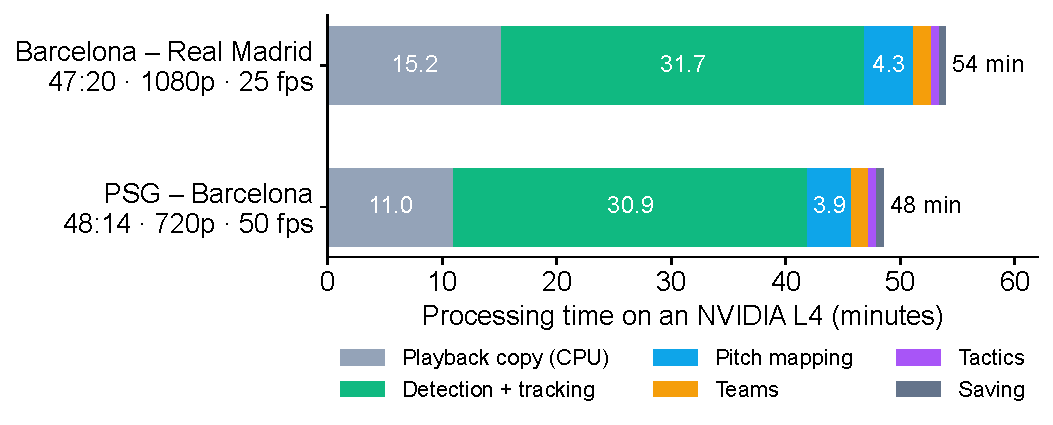
\includegraphics[width=0.9\textwidth]{long_video_stages}
	\caption{Processing time of the two halves per pipeline stage}
	\label{fig:long-stages}
\end{figure}

Processing took slightly more than real time on the L4, about 1.1 times the video length for the 25\,fps half and 1.0 times for the 50\,fps one, thanks to the frame-rate-aware stride. Detection and tracking dominate with about 31 minutes each. The second largest share, 11--15 minutes, is the H.264 playback copy, which runs on the pod's CPU. An earlier run of the first half on a different pod (a slice of an RTX PRO 6000 with a faster CPU) made the copy in 6.4 minutes and finished the whole half in 35 minutes, so the choice of machine matters as much as the GPU model. The GPU itself was barely used: at most 1.8\,GB of its 24\,GB of memory, so a much smaller and cheaper GPU would do. Peak RAM stayed below 4.5\,GB because frames are streamed. The dashboard handled the 54\,MB results file and the 1.2\,GB video without changes: the results are fetched once, and the video seeks immediately thanks to Range requests.

The distances of 55--63\,km per team over 47--48 minutes correspond to about 5.5--6.3\,km per outfield player-equivalent, in line with what professional players run in a half. The per-position top speeds are less convincing: their medians are 34.5 and 35.1\,km/h and the highest is 40.3\,km/h, above what players reach. On a 30-second clip, the top speed is the best one-second average of one player; over a half, a position's top speed is the best second out of 47 minutes, over several players and every tracking error in between, and one wrongly joined track or a wrong position in a fast camera pan is enough to set it. For full halves the distances are meaningful, while the top speed would need a statistic that one bad second cannot set, for example a high percentile instead of the maximum.

More valuable than the numbers was what the halves revealed about the pipeline. Nearly all the changes described in \autoref{sec:pipeline} after the first version came from these two runs: the upload limit and the chunked GPU upload, analysing the H.264 copy because OpenCV could not seek in AV1, the frame-rate-aware stride, the colour threshold for small players, the removal of people off the pitch, the ball selection, the referee detection, the joining of tracks, the position labels, the formation stability rule, the camera smoothing, and the protection against analysing a job twice. None of them showed up on the 30-second clips.

\section{Efficiency}

\autoref{tab:times} and \autoref{fig:performance} compare the processing times on the laptop and on the cloud GPU. The analysis is dominated by the two neural networks, so the GPU makes a large difference: a 30-second clip in Standard mode takes about 25 minutes on the laptop's CPU and 36--40 seconds on an L4. With the upload of the video and the download of the results, the total is about 53 seconds, still 28 times faster.

\begin{table}[H]
	\centering
	\begin{tabular}{|p{0.30\textwidth}|p{0.18\textwidth}|p{0.20\textwidth}|p{0.18\textwidth}|}
		\hline
		\textbf{Job} & \textbf{Laptop CPU (i7-1255U)} & \textbf{Docker on the laptop} & \textbf{Cloud GPU (L4)} \\
		\hline
		3\,s clip, Quick & 44--75\,s & 93\,s (207\,s first job) & 5\,s \\
		\hline
		30\,s clip, Standard & about 25\,min & not measured & 36--40\,s \\
		\hline
		47\,min half, Standard & not practical & not practical & 48--54\,min \\
		\hline
	\end{tabular}
	\caption{Processing times}
	\label{tab:times}
\end{table}

\begin{figure}[H]
	\centering
	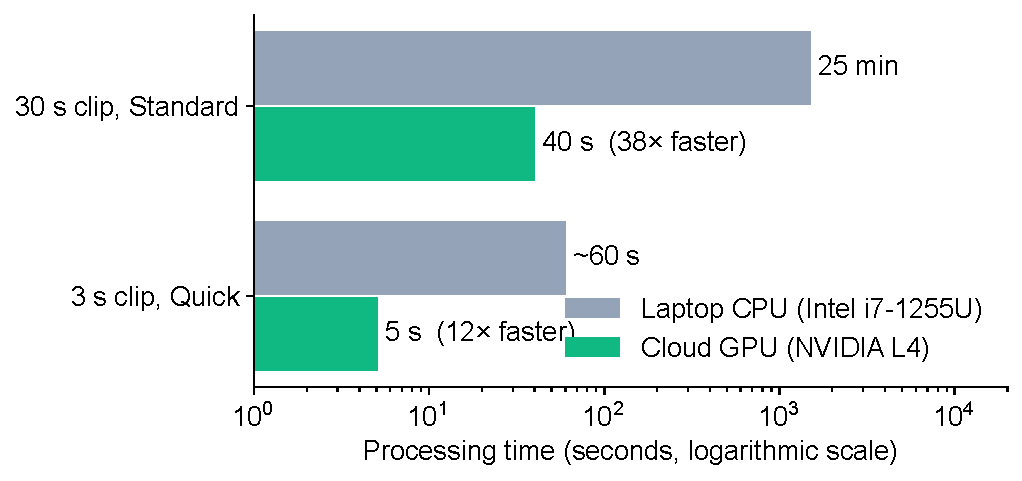
\includegraphics[width=0.85\textwidth]{performance}
	\caption{Processing time of the clips on the laptop CPU and on the cloud GPU (logarithmic scale)}
	\label{fig:performance}
\end{figure}

Three observations shaped the implementation. The first job after a worker starts is slower because the models are loaded; caching them per process means later jobs do not pay this again. Inside Docker on Windows the analysis was slower than natively, because the containers run in a WSL 2 virtual machine with a limited share of processor and memory. And the laptop's own GPU, a GeForce MX550 with 2\,GB, was about twice as slow as its CPU for these large models, which is why the worker defaults to the CPU and GPU work went to a rented machine. Laptop memory was a constraint of its own: with 7.7\,GB of RAM and the Docker stack running, two local analyses at the same time failed with out-of-memory errors while I was preparing the clean-up steps, so all local experiments ran one at a time.

\section{Scalability}

Workers share nothing but the queue and the storage, and the queue gives each job to exactly one worker, so throughput grows with the number of workers. More workers start with \texttt{docker compose --profile app up -d --scale worker=N} or on other machines, which then need access to the same storage, for example a network file system or object storage. The GPU service is stateless apart from its running jobs and can run on several machines. The API is stateless except for the Socket.IO rooms; several API instances behind a load balancer would need the Socket.IO Redis adapter so that events reach users connected to another instance. Processing time and the results file grow linearly with the video length: about 54\,MB per half, about 110\,MB for a full match, which the dashboard still loads as one file but which a future version could load in segments.

\section{Problems found during testing}

\autoref{tab:lessons} lists the defects that testing uncovered and the changes they led to. The first group comes from the first version on the demo clips, the second from the full halves and the new tests.

\begin{longtable}{|p{0.45\textwidth}|p{0.46\textwidth}|}
	\hline
	\textbf{Problem found} & \textbf{Change} \\
	\hline
	\endhead
	Uploaded clips did not play in the browser: the dataset uses a codec browsers do not support. & New stage: an H.264 playback copy at a constant frame rate, which also keeps the overlays frame-exact. \\
	\hline
	Two of five clips failed with ``out of range float values: nan'': for some camera angles the last matrix element is nearly zero. & Matrices are normalised by their norm with a fixed sign; non-finite numbers become \texttt{null}; regression test. \\
	\hline
	A team in a lime kit was not recognised: the fixed green range removed the shirts too. & The grass colour is measured around each player and compared in Lab space; two tests. \\
	\hline
	Goalkeepers were often labelled ``player'' and joined an outfield team. & Roles per track (25\,\% goalkeeper detections suffice); goalkeepers assigned by position. \\
	\hline
	The progress bar sometimes jumped backwards. & Database updates of each match are chained. \\
	\hline
	A re-analysis was accepted but nothing happened: BullMQ ignores a job whose ID still exists. & The finished job is removed before the new one is added. \\
	\hline
	The health check showed 0 workers while the Python worker ran. & Workers are counted from Redis's client list, accepting both naming schemes. \\
	\hline
	A top speed of 39.6\,km/h on clip 3. & Top speed as the best one-second average; regression test. \\
	\hline
	The laptop GPU was slower than its CPU. & CPU by default; optional cloud GPU with fallback. \\
	\hline
	\multicolumn{2}{|l|}{\textit{Found on the full halves and by the new tests}} \\
	\hline
	The first half was just over the 500\,MB upload limit, and RunPod's proxy may refuse a request body of that size. & Limit raised to 1\,GB; GPU upload in 50\,MB pieces with offsets and retries. \\
	\hline
	OpenCV failed to seek in the AV1 halves (``Corrupt frame detected''). & All stages read the H.264 playback copy. \\
	\hline
	The 50\,fps half would take twice as long as needed. & Stride scaled with the frame rate. \\
	\hline
	Far players ($8 \times 17$\,px) got no shirt colour; most of a team had no team. & Minimum shirt pixels relative to the player's size. \\
	\hline
	Substitutes and staff on the sidelines were marked as players. & Tracks usually more than 0.5\,m off the pitch are removed; test. \\
	\hline
	The main referee was counted as a player. & Referee kit learned from the assistants; players in that colour become referees; tests. \\
	\hline
	Spare balls and the penalty spot were taken for the ball (12\,\% of positions off the pitch). & Several candidates per frame, ball path followed on the pitch (\autoref{alg:ball}); tests. \\
	\hline
	Player numbers climbed to 1,423 over a half. & Broken tracks joined (555 left), then position labels (11 per team). \\
	\hline
	282 formation changes in one half. & A new formation must last 20 seconds (14 changes). \\
	\hline
	Movement paths darted across the video. & Camera model smoothed over 1.5\,s; test. \\
	\hline
	The CI system test failed after the results format changed to version 3. & The test was updated and now also checks the position labels. \\
	\hline
	The referee rule turned six goalkeepers of the demo clips into referees (found by the accuracy check). & Goalkeepers are only checked outside both penalty areas; regression test. \\
	\hline
	After the laptop slept, the queue handed the finished second half out again, and it was analysed twice. & ``Done'' note per job run; test. \\
	\hline
	\caption{Problems found during testing and the resulting changes}
	\label{tab:lessons}
\end{longtable}

The most useful lesson was that every new kind of footage exposed problems the previous tests could not have found. The codec, the camera angles and the kit colours were specific to the first real clips, and the sidelines, the spare balls, the referee and the identity problem only appeared over a full half. The five 30-second clips had made the pipeline look finished. Testing on long, real footage early, and turning each defect into a test, would have saved me the most time.

\section{Limitations and future work}
\label{sec:limitations}

The largest limitation is the single camera. Only what the broadcast camera shows is analysed, and players cannot be identified over a match, which is why the labels follow positions. Tactical-camera footage of the whole pitch, several camera angles, or shirt numbers read from higher-resolution video would allow named players and per-player statistics.

Two weaknesses only show over long videos. When only part of a team is visible, the slot matching can shift labels between neighbouring positions, and a position's top speed over a half is the single best second, which one tracking error can set (\autoref{sec:long-videos}). A high percentile instead of the maximum, and labels smoothed over longer periods, would make both less sensitive to single errors.

Events are missing entirely: passes, shots, tackles and possession are not detected. The distance between the ball and the nearest players over time would be a first step towards estimating possession and passes. The ball itself is found in only about half of the analysed frames of a full half; a model trained for small, fast objects, or a higher detection resolution around the ball's last known position, would help.

Processing a full half takes about as long as watching it on an L4, and the playback copy is encoded on the CPU, not the GPU. Splitting a match into segments that several workers analyse in parallel, and loading the results in time segments, would make full matches practical. The platform also runs on one machine; object storage instead of a shared folder, the Socket.IO Redis adapter and an orchestrator such as Kubernetes would spread it over several, and exporting queue length, processing times and error rates to a monitoring system would allow alerting.

Finally, the evaluation is small. The accuracy check covers 20 frames that I annotated myself. A larger set annotated by several people, or sensor tracking data, would measure positions, teams and especially identities over time far more reliably.
